\documentclass{article}
\usepackage[utf8]{inputenc}
\usepackage[T1]{fontenc}
\usepackage{geometry}
\RequirePackage[orthodox]{nag}
\usepackage{microtype}
\usepackage{booktabs}
\usepackage{mathptmx}
\usepackage{mathtools}
\usepackage{amssymb}
\usepackage{amsthm}
\usepackage{stmaryrd}
\usepackage{booktabs}
\usepackage{enumerate}
\usepackage{multirow}
\usepackage{nicefrac}
\usepackage{xspace}

\usepackage{algpseudocode}
\usepackage[colorlinks=true,linkcolor=blue]{hyperref}
\usepackage[colorinlistoftodos]{todonotes}

\allowdisplaybreaks

\theoremstyle{definition}
\newtheorem{Definition}{Definition}

\theoremstyle{plain}
\newtheorem{Thm}{Theorem}
\newtheorem{Conjecture}{Conjecture}
\newtheorem{Corollary}[Thm]{Corollary}
\newtheorem{Example}[Thm]{Example}
\newtheorem{Lemma}[Thm]{Lemma}
\newtheorem{Proposition}[Thm]{Proposition}
\newtheorem{Question}{Question}
\newtheorem{Remark}[Thm]{Remark}
\newtheorem{Theorem}[Thm]{Theorem}

\renewcommand{\mid}{\, \middle| \,}
\newcommand{\abs}[1]{\left| #1 \right|}
\newcommand{\menge}[1]{\ensuremath{\left\{ #1 \right\}}}
\newcommand{\set}[2]{\mbox{$ \left\{ \,#1 \mid #2 \,\right\}$}}
\newcommand{\ext}[1]{\llbracket #1  \rrbracket}
\newcommand{\fa}[2]{\forall {#1} \quad {#2}}
\newcommand{\ex}[2]{\exists {#1} \quad {#2}}

\DeclarePairedDelimiter\floor{\lfloor}{\rfloor}

\newcommand{\N}{\mathbb{N}}
\newcommand{\Q}{\mathbb{Q}}
\newcommand{\R}{\mathbb{R}}

\newcommand{\FCCS}{\textsc{fccs}}

\begin{document}
\author{Chris Wong}
\title{Frank Ramsey's Fantastic Numbers and Where to Find Them}
\maketitle

Ramsey's Theorem, introduced by the eponymous mathematician Frank P. Ramsey, is a fundamental result in combinatorics and graph theory. It states that any sufficiently large graph must always contain one of two subgraphs: either a \textit{clique} or a \textit{stable set}. However, Ramsey's proof of this theorem does not tell us precisely how large the graph must be---only that this threshold is finite. The minimum number of vertices needed to satisfy Ramsey's Theorem is called a \textit{Ramsey number}, and finding the values of these numbers is an active topic of research. We summarise existing results on Ramsey numbers, along with some common techniques used to derive them.

\section{Preliminaries}

Before we introduce the Ramsey numbers, we must first define a few terms.

A \textit{graph} $G = (V, E)$ consists of a set of \textit{vertices} $V$ connected by a set of \textit{edges} $E \subseteq \{\, \{u, v\} \mid u, v \in V \,\}$. The elements of an edge $e$ are called its \textit{endpoints}. For the purposes of this paper, we assume that the graphs are \textit{simple}: that is, every pair of vertices has at most one edge between them.

A graph is \textit{complete} when every pair of vertices is connected by an edge. For each positive integer $n$, the complete graph on $n$ vertices is unique and denoted $K_n$.

An \textit{subgraph} $G'$ of $G$ is formed from a subset of the vertices and edges of $G$. The vertex subset must include all endpoints of the edge subset, but may also contain extra vertices. In a \textit{vertex-induced} subgraph, $e$ is an edge of $G'$ if and only if its endpoints are also in $G'$. When a subgraph is complete, it is called a \textit{clique}. Conversely, if no pair of vertices in a vertex-induced subgraph has an edge between them, then the subgraph is a \textit{stable set}.

An \textit{edge colouring} labels every edge of a graph by elements from a given set of colours. In this report, we will use the two colours \textit{red} and \textit{blue}.

With these definitions, we can state Ramsey's Theorem, and with it, define the Ramsey numbers:

\begin{Theorem}[Ramsey's Theorem for red-blue colourings] \label{ramseys_theorem}
    Let $s$ and $t$ be positive integers. Then for sufficiently large $n$, every red-blue edge colouring of $K_n$ either has a clique of size $s$ all coloured red, or a clique of size $t$ all coloured blue.
\end{Theorem}

\begin{Definition}[Ramsey numbers]
    Define $R(s,t)$ as the smallest $n$ such that the conclusion of \cref{ramseys_theorem} holds. This is the \textit{Ramsey number} of $(s,t)$.
\end{Definition}

There is an alternative statement of the theorem in terms of \textit{cliques} and \textit{stable sets}:

\begin{Theorem}[Ramsey's Theorem for cliques and stable sets]
    Let $s$ and $t$ be positive integers. Then for sufficiently large $n$, every simple graph on $n$ vertices either has a clique of size $n$, or a stable set of size $t$.
\end{Theorem}

It can be shown that the two statements are equivalent.

\section{1-fish, 2-fish, red fish, blue fish}

As with other concepts in mathematics, Ramsey numbers have their simple cases: namely, the values of $R(1,t)$ and $R(2,t)$. These cases are easy to state and prove, and so are given below.

\begin{Proposition}
    For any positive $s$ and $t$,
    \[ R(s,1) = R(1,t) = 1 \ . \]
\end{Proposition}

\begin{proof}
    Observe that a clique with one vertex has no edges. Hence, trivially, all of its edges are coloured both red and blue. The smallest complete graph with a one-vertex clique is $K_1$ itself. The proposition follows.
\end{proof}

\begin{Proposition}
    For any positive $t$,
    \[ R(2,t) = t \ . \]
\end{Proposition}

\begin{proof}
    Consider a colouring of $K_t$. If every edge is coloured blue, then the graph has a blue clique of size $t$; and we are done.

    Otherwise, there must exist at least one edge coloured red. Take one such edge, along with the two vertices incident to it. This is a red clique of size 2.
\end{proof}

On learning these results, one may wonder: is the expression for $R(3,t)$ as simple as the two before it? The answer is no---we have only approximate bounds for numbers of this form. Mathematician Jeong Han Kim received a Fulkerson Prize for the following result.

\begin{Theorem}[\citet{RSA:RSA3240070302}] \label{kims_theorem}
    For sufficiently large $t$, the value of $R(3,t)$ is within a constant factor of $t^2/\log t$.
\end{Theorem}

Kim's argument is much more elaborate than those for $R(1,t)$ and $R(2,t)$; for brevity the proof is omitted. It uses the so-called \textit{R\"{o}dl's nibble method}: a probabilistic argument which constructs the desired colouring in small random increments, or ``nibbles''. While R\"{o}dl's method is out of scope for this article, we will cover probabilistic techniques in general in \cref{probabilistic_method}.

Finally, we observe that the colours \emph{red} and \emph{blue} are interchangeable: any colouring that satisfies the Ramsey property for $(s,t)$ can be adapted to one for $(t,s)$ by swapping the colours.

\begin{Proposition}
    For any positive $s$ and $t$,
    \[ R(s,t) = R(t,s) \ . \]
\end{Proposition}

\begin{proof}
    By symmetry of the edge colouring.
\end{proof}

\section{Computing Ramsey numbers}

The definition of Ramsey numbers is easy to state. What is surprising, then, is how difficult they are to compute. As of this writing, the last exact result was proved by \cite{JGT:JGT3190190304}, who showed that $R(4,5) = 25$. The value of $R(5,5)$---just one step above---is still an open problem!

\begin{table}
    \centering
    \begin{tabular}{ccccccccc}
        \toprule
        s \textbackslash\ t & 3 & 4 & 5 & 6 & 7 & 8 & 9 \\
        \midrule
        3 & 6 & 9 & 14 & 18 & 23 & 28 & 36 \\
        4 & & 18 & 25 & 36--41 & 49--61 & 58--84 & 73--115 \\
        5 & & & 43--49 & 58--87 & 80--143 & 101--216 & 126--316 \\
        6 & & & & 102--165 & 113--298 & 132-495 & 169--780 \\
        7 & & & & & 205--540 & 217--1031 & 241--1713 \\
        8 & & & & & & 282--1870 & 317--3583 \\
        9 & & & & & & & 565--6588 \\
        \bottomrule
    \end{tabular}
    \caption{Table of known values and bounds for Ramsey numbers $R(s,t)$, for $3 \leq s \leq t \leq 9$. The bounds are inclusive: we read that $43 \leq R(5,5) \leq 49$. Adapted from \cite{radziszowski1994small}.}
\end{table}

This difficulty stems from the sheer number of colourings that must be checked. Since a Ramsey number is a statement about \emph{all} colourings of a particular graph, it is not enough to find a single example---we have to account for them all. Moreover, as the number of possible colourings grows exponentially with the number of vertices, it is not feasible to check every colouring for all but trivial values of $s$ and $t$. For this reason, while we do know specific cases, there is no known efficient algorithm for computing Ramsey numbers in general.

\section{Upper and lower bounds}

As it can be difficult to compute a Ramsey number exactly, most research instead focuses on deriving upper and lower bounds. These bounds may apply to a family of Ramsey numbers---for example, \cref{kims_theorem} is a bound on $R(3,t)$---or it may apply to only a particular one. Either way, they can be an important step toward finding an exact result. In particular, if we can show that $R(s,t) \geq n$ and $R(s,t) \leq n$ for the same $n$, then it follows that $R(s,t) = n$.

To prove a lower bound for a Ramsey number---that is, $R(s,t) > n$---we only need a counterexample: a colouring on $K_n$ which does \emph{not} have a red clique of size $s$ or a blue clique of size $t$. This colouring is called a \textit{Ramsey graph} of size $n$. Since a Ramsey number is a statement about all colourings on $K_n$, such a colouring is sufficient to show that $R(s,t) \nleq n$, hence $R(s,t) > n$.

\begin{figure}
    \centering
    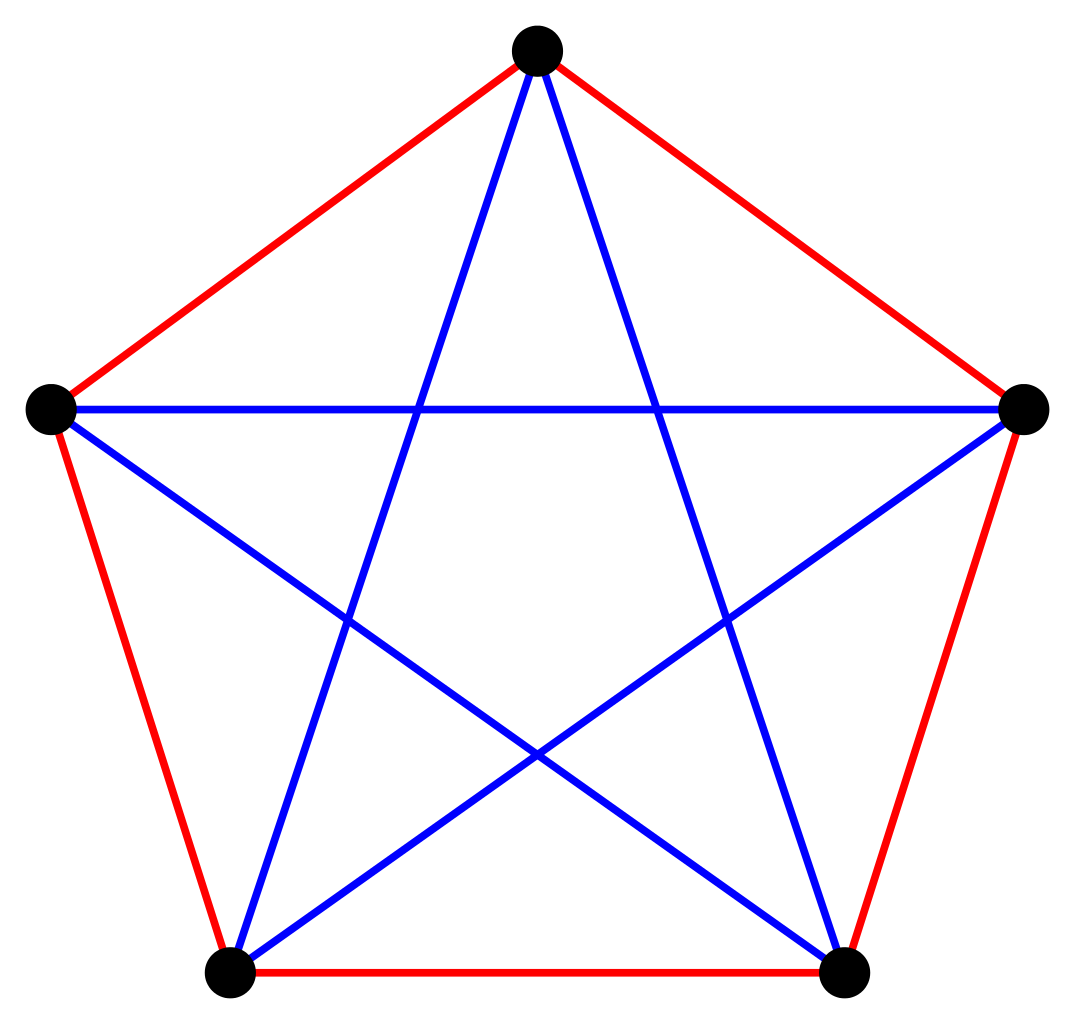
\includegraphics[width=0.3\textwidth]{RamseyTheory_K5_no_mono_K3.png}
    \caption{This edge colouring of $K_5$ has no red clique of size 3, nor a blue clique of size 3. It then follows that $R(3,3) > 5$. (Image by Richtom80 on Wikipedia.)}
\end{figure}

On the other hand, to prove an upper bound is often more difficult. This is because to show that $R(s,t) \leq n$, we must prove that \emph{all} colourings on $K_n$ have the desired property.

That is not to say that lower bounds are not hard to find. For all but trivial values for $s$ and $t$, the set of possible colourings is too large to search exhaustively. Finding a counterexample at this scale often requires special techniques: in \citet{exoo2004some}, Ramsey graphs are constructed from non-abelian groups. Moreover, to prove a \emph{general} lower bound often involves non-constructive techniques. In the next section we derive such a bound for $R(k,k)$, using the non-constructive probabilistic method.

\section{The probabilistic method}

\label{probabilistic_method}

One interesting aspect of Ramsey numbers, as well as graph theory as a whole, is the breadth of techniques used in its proofs. Past practitioners have taken ideas from differential equations and probability theory, and used computational methods to narrow down their results. The approximation $R(3,t) \sim t^2/\log t$, as we saw earlier in \cref{kims_theorem}, was proved using probability and differential equations; the bound $R(4,6) \leq 41$ by \citet{mckay1997subgraph} was partly derived using counting arguments, with computer-assisted linear programming completing their proof.

For this report, we will focus on one such technique: the \textit{probabilistic method}, pioneered by Paul Erdős in \citeyear{erdos1947some}. The key idea is to define a random process that builds a colouring, and show the probability that the Ramsey property holds is less than one. From this, it must follow that there exists a colouring where this property does \emph{not} hold.

This argument is non-constructive: it shows that such a counterexample exists, but does not tell us what it is. Despite this caveat, the method is valid and its conclusion is correct with no chance of error.

To illustrate the probabilistic method, we give a proof of the lower bound $R(k,k) \geq 2^{\frac k 2}$. This proof depends on a short lemma, which we will introduce first.

\begin{Lemma} \label{binomial_bound}
    For all positive integers $n$ and $k$,
    \[ {n \choose k} \leq \frac{n^k}{2^{k-1}} \ . \]
\end{Lemma}

\begin{proof}
    Expanding the definition of the binomial coefficient, we see that
    \[
        {n \choose k}
        = \frac{n!}{(n-k)!k!}
        = \frac{n(n-1)\ldots(n-(k-1))}{k!}
        \leq \frac{n^k}{k!} \ .
    \]
    To complete the proof, we observe that
    \[
        2^{k-1}
        = 1 \times 2 \times 2 \times \ldots \times 2
        \leq 1 \times 2 \times 3 \times \ldots \times k
        = k! \ ;
    \]
    it then follows that
    \[
        {n \choose k} \leq \frac{n^k}{2^{k-1}} \ . \qedhere
    \]
\end{proof}

\begin{Theorem}[\cite{erdos1947some}]
    For all $k \geq 2$, the following lower bound holds for the Ramsey numbers:
    \[ R(k,k) \geq 2^{\frac k 2} \ . \]
\end{Theorem}

\begin{proof}\citep{aigner2010proofs}.
    Let $k \geq 2$. Consider the complete graph $K_n$ on $n$ vertices, where $n < 2^{\frac k 2}$. Since every pair of vertices in this graph is connected by an edge, there must be $n \choose 2$ edges in total.

    Now, suppose that each edge is coloured red or blue independently with probability $\frac 1 2$. As each of these $2^{n \choose 2}$ colourings is equally likely, the probability of choosing a particular colouring is $2^{-{n \choose 2}}$.

    Let $A$ be a subset of vertices of size $k$. The probability of the event $A_\red$ that all edges within $A$ are coloured red is then $2^{-{k \choose 2}}$. Hence it follows that the probability $p_\red$ that \emph{some} $k$-set is coloured all red is bounded by
    \[
        p_\red = \Pr(\bigcup_{\abs{A} = k} A_\red)
        \leq \sum_{\abs{A} = k} \Pr(A_\red)
        = {n \choose k} 2^{-{k \choose 2}} \ .
    \]

Now, applying \cref{binomial_bound}, we use the fact that $n < 2^{\frac k 2}$ to conclude that
    \[
        {n \choose k} 2^{-{k \choose 2}}
        \leq \frac{n^k}{2^{k-1}} 2^{-{k \choose 2}}
        < 2^{\frac{k^2}{2} - {k \choose 2} - k + 1}
        = 2^{-\frac k 2 + 1}
        \leq \frac 1 2 \ .
    \]

Hence $p_\red < \frac 1 2$, and by symmetry $p_\blue < \frac 1 2$ for the probability that some $k$ vertices have all edges between them coloured blue. It follows that $p_\red + p_\blue < 1$, so there must exist a colouring with no red or blue $K_k$. This means that $K_n$ does not have the Ramsey property for $(k, k)$, and the Ramsey number $R(k,k) \geq 2^{\frac k 2}$.
\end{proof}

\section{Conclusion}

In a way, Ramsey numbers are the perfect mathematical problem. Their definition is easy to state, but the values themselves are difficult to derive for all but trivial cases. In the course of proving a result, one draws from areas as diverse as differential equations, probability theory, and linear programming. As the great Paul Erdős once said:

\begin{displayquote}
    Suppose aliens invade the earth and threaten to obliterate it in a year's time unless human beings can find the Ramsey number for red five and blue five [$R(5,5)$]. We could marshal the world's best minds and fastest computers, and within a year we could probably calculate the value. If the aliens demanded the Ramsey number for red six and blue six [$R(6,6)$], however, we would have no choice but to launch a preemptive attack.
\end{displayquote}

The author is inclined to agree.

\bibliographystyle{abbrvnat}
\bibliography{sources}

\end{document}
